\documentclass{esannV2}
\usepackage{graphicx}
%\usepackage[dvips]{graphicx}
%\usepackage[latin1]{inputenc}
\usepackage[utf8]{inputenc}
\usepackage{amssymb,amsmath,array}
\usepackage{color}
\usepackage[ruled,linesnumbered,lined]{algorithm2e}

%    Q-circuit version 2
%    Copyright (C) 2004  Steve Flammia & Bryan Eastin
%    Last modified on: 9/16/2011
%
%    This program is free software; you can redistribute it and/or modify
%    it under the terms of the GNU General Public License as published by
%    the Free Software Foundation; either version 2 of the License, or
%    (at your option) any later version.
%
%    This program is distributed in the hope that it will be useful,
%    but WITHOUT ANY WARRANTY; without even the implied warranty of
%    MERCHANTABILITY or FITNESS FOR A PARTICULAR PURPOSE.  See the
%    GNU General Public License for more details.
%
%    You should have received a copy of the GNU General Public License
%    along with this program; if not, write to the Free Software
%    Foundation, Inc., 59 Temple Place, Suite 330, Boston, MA  02111-1307  USA

% Thanks to the Xy-pic guys, Kristoffer H Rose, Ross Moore, and Daniel Müllner,
% for their help in making Qcircuit work with Xy-pic version 3.8.  
% Thanks also to Dave Clader, Andrew Childs, Rafael Possignolo, Tyson Williams,
% Sergio Boixo, Cris Moore, Jonas Anderson, and Stephan Mertens for helping us test 
% and/or develop the new version.

\usepackage{xy}
\xyoption{matrix}
\xyoption{frame}
\xyoption{arrow}
\xyoption{arc}

\usepackage{ifpdf}
\ifpdf
\else
\PackageWarningNoLine{Qcircuit}{Qcircuit is loading in Postscript mode.  The Xy-pic options ps and dvips will be loaded.  If you wish to use other Postscript drivers for Xy-pic, you must modify the code in Qcircuit.tex}
%    The following options load the drivers most commonly required to
%    get proper Postscript output from Xy-pic.  Should these fail to work,
%    try replacing the following two lines with some of the other options
%    given in the Xy-pic reference manual.
\xyoption{ps}
\xyoption{dvips}
\fi

% The following resets Xy-pic matrix alignment to the pre-3.8 default, as
% required by Qcircuit.
\entrymodifiers={!C\entrybox}

\newcommand{\bra}[1]{{\left\langle{#1}\right\vert}}
\newcommand{\ket}[1]{{\left\vert{#1}\right\rangle}}
    % Defines Dirac notation. %7/5/07 added extra braces so that the commands will work in subscripts.
\newcommand{\qw}[1][-1]{\ar @{-} [0,#1]}
    % Defines a wire that connects horizontally.  By default it connects to the object on the left of the current object.
    % WARNING: Wire commands must appear after the gate in any given entry.
\newcommand{\qwx}[1][-1]{\ar @{-} [#1,0]}
    % Defines a wire that connects vertically.  By default it connects to the object above the current object.
    % WARNING: Wire commands must appear after the gate in any given entry.
\newcommand{\cw}[1][-1]{\ar @{=} [0,#1]}
    % Defines a classical wire that connects horizontally.  By default it connects to the object on the left of the current object.
    % WARNING: Wire commands must appear after the gate in any given entry.
\newcommand{\cwx}[1][-1]{\ar @{=} [#1,0]}
    % Defines a classical wire that connects vertically.  By default it connects to the object above the current object.
    % WARNING: Wire commands must appear after the gate in any given entry.
\newcommand{\gate}[1]{*+<.6em>{#1} \POS ="i","i"+UR;"i"+UL **\dir{-};"i"+DL **\dir{-};"i"+DR **\dir{-};"i"+UR **\dir{-},"i" \qw}
    % Boxes the argument, making a gate.
\newcommand{\meter}{*=<1.8em,1.4em>{\xy ="j","j"-<.778em,.322em>;{"j"+<.778em,-.322em> \ellipse ur,_{}},"j"-<0em,.4em>;p+<.5em,.9em> **\dir{-},"j"+<2.2em,2.2em>*{},"j"-<2.2em,2.2em>*{} \endxy} \POS ="i","i"+UR;"i"+UL **\dir{-};"i"+DL **\dir{-};"i"+DR **\dir{-};"i"+UR **\dir{-},"i" \qw}
    % Inserts a measurement meter.
    % In case you're wondering, the constants .778em and .322em specify
    % one quarter of a circle with radius 1.1em.
    % The points added at + and - <2.2em,2.2em> are there to strech the
    % canvas, ensuring that the size is unaffected by erratic spacing issues
    % with the arc.
\newcommand{\measure}[1]{*+[F-:<.9em>]{#1} \qw}
    % Inserts a measurement bubble with user defined text.
\newcommand{\measuretab}[1]{*{\xy*+<.6em>{#1}="e";"e"+UL;"e"+UR **\dir{-};"e"+DR **\dir{-};"e"+DL **\dir{-};"e"+LC-<.5em,0em> **\dir{-};"e"+UL **\dir{-} \endxy} \qw}
    % Inserts a measurement tab with user defined text.
\newcommand{\measureD}[1]{*{\xy*+=<0em,.1em>{#1}="e";"e"+UR+<0em,.25em>;"e"+UL+<-.5em,.25em> **\dir{-};"e"+DL+<-.5em,-.25em> **\dir{-};"e"+DR+<0em,-.25em> **\dir{-};{"e"+UR+<0em,.25em>\ellipse^{}};"e"+C:,+(0,1)*{} \endxy} \qw}
    % Inserts a D-shaped measurement gate with user defined text.
\newcommand{\multimeasure}[2]{*+<1em,.9em>{\hphantom{#2}} \qw \POS[0,0].[#1,0];p !C *{#2},p \drop\frm<.9em>{-}}
    % Draws a multiple qubit measurement bubble starting at the current position and spanning #1 additional gates below.
    % #2 gives the label for the gate.
    % You must use an argument of the same width as #2 in \ghost for the wires to connect properly on the lower lines.
\newcommand{\multimeasureD}[2]{*+<1em,.9em>{\hphantom{#2}} \POS [0,0]="i",[0,0].[#1,0]="e",!C *{#2},"e"+UR-<.8em,0em>;"e"+UL **\dir{-};"e"+DL **\dir{-};"e"+DR+<-.8em,0em> **\dir{-};{"e"+DR+<0em,.8em>\ellipse^{}};"e"+UR+<0em,-.8em> **\dir{-};{"e"+UR-<.8em,0em>\ellipse^{}},"i" \qw}
    % Draws a multiple qubit D-shaped measurement gate starting at the current position and spanning #1 additional gates below.
    % #2 gives the label for the gate.
    % You must use an argument of the same width as #2 in \ghost for the wires to connect properly on the lower lines.
\newcommand{\control}{*!<0em,.025em>-=-<.2em>{\bullet}}
    % Inserts an unconnected control.
\newcommand{\controlo}{*+<.01em>{\xy -<.095em>*\xycircle<.19em>{} \endxy}}
    % Inserts a unconnected control-on-0.
\newcommand{\ctrl}[1]{\control \qwx[#1] \qw}
    % Inserts a control and connects it to the object #1 wires below.
\newcommand{\ctrlo}[1]{\controlo \qwx[#1] \qw}
    % Inserts a control-on-0 and connects it to the object #1 wires below.
\newcommand{\targ}{*+<.02em,.02em>{\xy ="i","i"-<.39em,0em>;"i"+<.39em,0em> **\dir{-}, "i"-<0em,.39em>;"i"+<0em,.39em> **\dir{-},"i"*\xycircle<.4em>{} \endxy} \qw}
    % Inserts a CNOT target.
\newcommand{\qswap}{*=<0em>{\times} \qw}
    % Inserts half a swap gate.
    % Must be connected to the other swap with \qwx.
\newcommand{\multigate}[2]{*+<1em,.9em>{\hphantom{#2}} \POS [0,0]="i",[0,0].[#1,0]="e",!C *{#2},"e"+UR;"e"+UL **\dir{-};"e"+DL **\dir{-};"e"+DR **\dir{-};"e"+UR **\dir{-},"i" \qw}
    % Draws a multiple qubit gate starting at the current position and spanning #1 additional gates below.
    % #2 gives the label for the gate.
    % You must use an argument of the same width as #2 in \ghost for the wires to connect properly on the lower lines.
\newcommand{\ghost}[1]{*+<1em,.9em>{\hphantom{#1}} \qw}
    % Leaves space for \multigate on wires other than the one on which \multigate appears.  Without this command wires will cross your gate.
    % #1 should match the second argument in the corresponding \multigate.
\newcommand{\push}[1]{*{#1}}
    % Inserts #1, overriding the default that causes entries to have zero size.  This command takes the place of a gate.
    % Like a gate, it must precede any wire commands.
    % \push is useful for forcing columns apart.
    % NOTE: It might be useful to know that a gate is about 1.3 times the height of its contents.  I.e. \gate{M} is 1.3em tall.
    % WARNING: \push must appear before any wire commands and may not appear in an entry with a gate or label.
\newcommand{\gategroup}[6]{\POS"#1,#2"."#3,#2"."#1,#4"."#3,#4"!C*+<#5>\frm{#6}}
    % Constructs a box or bracket enclosing the square block spanning rows #1-#3 and columns=#2-#4.
    % The block is given a margin #5/2, so #5 should be a valid length.
    % #6 can take the following arguments -- or . or _\} or ^\} or \{ or \} or _) or ^) or ( or ) where the first two options yield dashed and
    % dotted boxes respectively, and the last eight options yield bottom, top, left, and right braces of the curly or normal variety.  See the Xy-pic reference manual for more options.
    % \gategroup can appear at the end of any gate entry, but it's good form to pick either the last entry or one of the corner gates.
    % BUG: \gategroup uses the four corner gates to determine the size of the bounding box.  Other gates may stick out of that box.  See \prop.

\newcommand{\rstick}[1]{*!L!<-.5em,0em>=<0em>{#1}}
    % Centers the left side of #1 in the cell.  Intended for lining up wire labels.  Note that non-gates have default size zero.
\newcommand{\lstick}[1]{*!R!<.5em,0em>=<0em>{#1}}
    % Centers the right side of #1 in the cell.  Intended for lining up wire labels.  Note that non-gates have default size zero.
\newcommand{\ustick}[1]{*!D!<0em,-.5em>=<0em>{#1}}
    % Centers the bottom of #1 in the cell.  Intended for lining up wire labels.  Note that non-gates have default size zero.
\newcommand{\dstick}[1]{*!U!<0em,.5em>=<0em>{#1}}
    % Centers the top of #1 in the cell.  Intended for lining up wire labels.  Note that non-gates have default size zero.
\newcommand{\Qcircuit}{\xymatrix @*=<0em>}
    % Defines \Qcircuit as an \xymatrix with entries of default size 0em.
\newcommand{\link}[2]{\ar @{-} [#1,#2]}
    % Draws a wire or connecting line to the element #1 rows down and #2 columns forward.
\newcommand{\pureghost}[1]{*+<1em,.9em>{\hphantom{#1}}}
    % Same as \ghost except it omits the wire leading to the left. 


%***********************************************************************
% !!!! IMPORTANT NOTICE ON TEXT MARGINS !!!!!
%***********************************************************************
%
% Please avoid using DVI2PDF or PS2PDF converters: some undesired
% shifting/scaling may occur when using these programs
% It is strongly recommended to use the DVIPS converters, and to submit
% PS file. You may submit a PDF file if and only if you use ADOBE ACROBAT
% to convert your PS file to PDF.
%
% Check that you have set the paper size to A4 (and NOT to letter) in your
% dvi2ps converter, in Adobe Acrobat if you use it, and in any printer driver
% that you could use.  You also have to disable the 'scale to fit paper' option
% of your printer driver.
%
% In any case, please check carefully that the final size of the top and
% bottom margins is 5.2 cm and of the left and right margins is 4.4 cm.
% It is your responsibility to verify this important requirement.  If these margin requirements and not fulfilled at the end of your file generation process, please use the following commands to correct them.  Otherwise, please do not modify these commands.
%
\voffset 0 cm \hoffset 0 cm \addtolength{\textwidth}{0cm}
\addtolength{\textheight}{0cm}\addtolength{\leftmargin}{0cm}

%***********************************************************************
% !!!! USE OF THE esannV2 LaTeX STYLE FILE !!!!!
%***********************************************************************
%
% Some commands are inserted in the following .tex example file.  Therefore to
% set up your ESANN submission, please use this file and modify it to insert
% your text, rather than staring from a blank .tex file.  In this way, you will
% have the commands inserted in the right place.

\begin{document}
%style file for ESANN manuscripts
\title{Quantum one-class classification with a distance-based classifier}

%***********************************************************************
% AUTHORS INFORMATION AREA
%***********************************************************************
\author{Nicolas M. de Oliveira and Adenilton J. da Silva and Teresa B. Ludermir
%
% Optional short acknowledgment: remove next line if non-needed
\thanks{This work is supported by research grants from CNPq, CAPES and FACEPE (Brazilian research agencies).}
%
% DO NOT MODIFY THE FOLLOWING '\vspace' ARGUMENT
\vspace{.3cm}\\
%
% Addresses and institutions (remove "1- " in case of a single institution)
Universidade Federal de Pernambuco \\
Centro de Informática \\
Cidade Universitária - 50740-560 - Recife/PE - Brazil
}
%***********************************************************************
% END OF AUTHORS INFORMATION AREA
%***********************************************************************

\maketitle

\begin{abstract}
Classify new inputs of a dataset is one of the most known problems in machine learning. Recently, some attention has been paid to solving this kind of problem in the quantum computing paradigm. In this paper, we will show how to use a distance-based classifier to perform one-class classification on a NISQ computer. Experimental results were obtained by running the proposed classifier on a computer provided by IBM Quantum Experience.
\end{abstract}

\section{Introduction}

Quantum computing is a field that is being highly explored because of its possible ability to solve certain problems more efficiently than in classical computers. Examples of this higher efficiency compared to classical computing are the Shor's algorithm \cite{shor1994} and the Grover's algorithm \cite{grover1996}. Peculiar characteristics such as quantum parallelism, and other phenomena only observed in quantum mechanics, make the application of such computational paradigm to problems for which no efficient algorithmic solutions are known to arouse the interest of many researchers. A more complete study of quantum characteristics and phenomena can be found in \cite{nielsen2010quantum}.

It is the possibility of quantum superposition of qubit states that allows quantum parallelism to be achieved. And it's this parallelism that can make the quantum computer an efficient alternative to classical computers with respect to the execution of exponential order algorithms (classically) in polynomial time. Thus, it is natural for quantum computing to be employed in areas of computing that demand more processing power. It is in this context that the interest in \textit{Quantum Machine Learning} (QML) arises.

Techniques for performing QML have been studied previously in several occasions. Many of these works make use of quantum computing to deal with supervised learning problems: a quantum support vector machine implementation is given in \cite{rebentrost2014quantum}; in \cite{kapoor2016quantum} the authors were able to improve learning for a perceptron through quantum amplitude amplification; in \cite{schuld2016prediction} a supervised pattern recognition algorithm that implements a linear regression model in quantum computers was developed.

In this paper, we investigate the \textit{Distance-based Quantum Classifier} (DBQC) proposed by \cite{schuld2017implementing} and present a modification to this classifier to allow its implementation on NISQ (\textit{Noisy Intermediate-Scale Quantum Computing}) computers \cite{Preskill2018quantumcomputingin}. Such modification was inspired by \textit{Probabilistic Quantum Memories} (PQM) \cite{trugenberger2001probabilistic} and aims to solve the impossibility of classifying samples of \textit{class 2} (qubit class $|1\rangle$), due to its rapid decoherence \cite{schuld2017implementing}. Experiments were done on IBM Quantum Experience \cite{ibmq} to validate our classifier, first in an error-free simulation environment and then on the non-error-corrected hardware of five superconducting qubits (specifically \textit{ibmq\_vigo}). We obtained good results by executing our approach on a real quantum machine and thus showed that our classifier can get around the problem of the original classifier.

The remainder of this paper is divided in 4 sections. Section 2 describes the original classifier that motivated our proposal. Section 3 presents the main results of this work: a description of our quantum on-class classifier. Section 4 presents details of the experiments performed as well as the results obtained and a brief discussion about them. Finally, Section 5 is the conclusion.

\section{Distance-based quantum classifier}

The Distance-based Quantum Classifier (DBQC) proposed by \cite{schuld2017implementing} aims to investigate how to perform a distance-based classification task from the construction of a simple quantum circuit. The strategy used in DQBC is basically to use \textit{amplitude encoding} to encode the input features and quantum interference to evaluate the distance from a new input vector to the training set vectors. Such a construction aims to provide a simple classification model that can be implemented in existing quantum devices.

To validate the DBQC, the authors performed supervised classification experiments using the Iris dataset \cite{fisher1936use}. The quantum system that performs the classification is shown in Equation~\ref{eq:dbqc_state}. Where $|m\rangle$ is an index register flagging the $m$th training vector, $|\psi_{\mathbf{x}^m}\rangle$ is the $m$th training vector, $|\psi_{\tilde{\mathbf{x}}}\rangle$ is the new input and $|y^m\rangle$ is a single qubit that stores the vector class.

\begin{equation}
|\mathcal{D}\rangle = \frac{1}{\sqrt{2 M}} \sum_{m=1}^M |m\rangle \Big( |0\rangle |\psi_{\tilde{\mathbf{x}}}\rangle + |1\rangle |\psi_{\mathbf{x}^m}\rangle \Big) |y^m\rangle
\label{eq:dbqc_state}
\end{equation}

The main point of DBQC lies in a conditional measurement operation that depends on the probability of measuring $|0\rangle$ in the \textit{ancilla qubit}. The probability of success of this postselection is $p_{acc}=\frac{1}{4M}\sum_m|\tilde{\mathbf{x}} + \mathbf{x}^{m}|^2$ and it's around 0.5. A measurement is made in the \textit{class qubit} only after the postselection succeeds. Experimental results showed 100\% accuracy for classes 1 and 2 of the Iris dataset. However, it is important to say that accuracy considers only those experiments whose postselection was successful (i.e., with probability greater than 0.5). In addition, the authors stress that due to the rapid decoherence of the \textit{class qubit} storing $|1\rangle$ it was impossible to classify new input vectors from class 2 and therefore only input vectors from class 1 were presented.

\section{Quantum one-class classifier}

The postselection of the DBQC \cite{schuld2017implementing} succeeds with probability $p_{acc}=\frac{1}{4M}\sum_m|\tilde{\mathbf{x}} + \mathbf{x}^{m}|^2$.  This probability depends on data distribution and can tend to zero. Figure~\ref{fig:example_pacc} presents an artificial example of dataset where the postselection probability is approximately 0.02 for the pattern $\mathbf{x}_0$ and 0.98 for pattern $\mathbf{x}_1$. The postselection probability is a function of the Euclidean distance of the new pattern to the patterns in the dataset and returns 0 with higher probability if the new pattern is near to the patterns in the dataset. In this Section, we redefine the DBQC to use the outcome of the postselection as the output of the classifier. With this modification, we remove the \textit{class qubit}, reduce the number of repetitions necessary to estimate the output of the classifier and reduces the number of operations necessary to perform the classification.

\begin{figure}[ht]
    \centering
    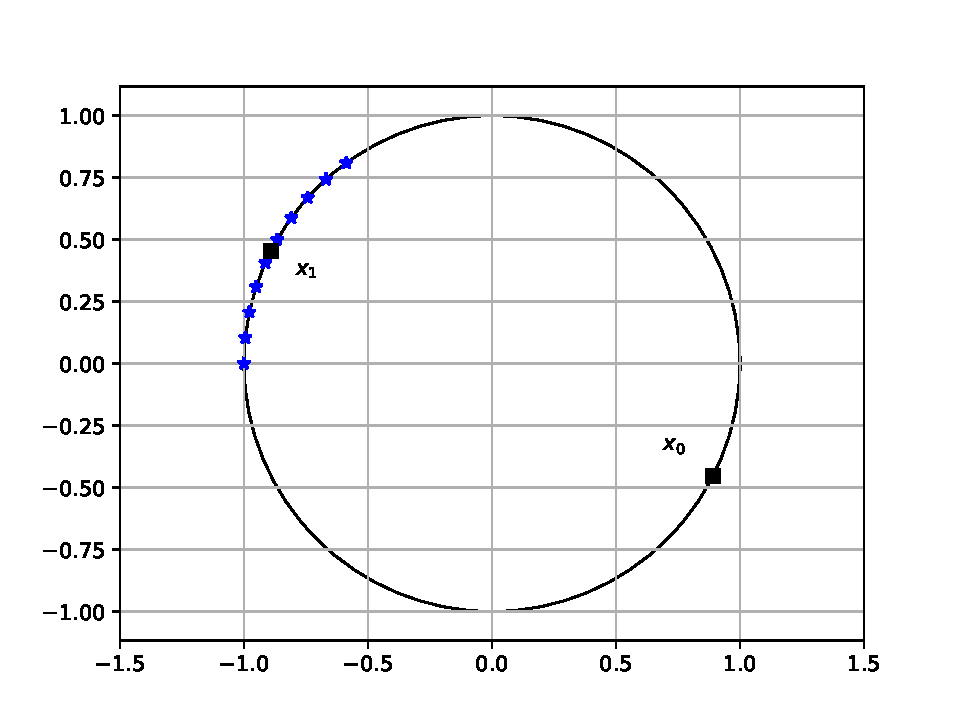
\includegraphics[scale=0.4]{fig1}
    \caption{Artificial example where the probability of postselection tends to zero for a given new input vector.}
    \label{fig:example_pacc}
\end{figure}

The classifier proposed here in this paper was based on the DBQC and extends its results to allow the classification of a new input vector from a quantum one-class classifier indicating the probability that the vector will be associated with the set of loaded (training) vectors in the classifier. Such a modification allows us to work around the problem of rapid decoherence pointed out by \cite{schuld2017implementing} and correctly classify samples of \textit{class 2} (qubit class $|1\rangle$) on real NISQ computers.

In our approach we use the same data preprocessing strategy used in \cite{schuld2017implementing}. As with the original classifier, we use the quantum rotation gate $R_{y}$ (Equation~\ref{eq:ry}) to load training vectors and new input vectors. However, the classification of a new input vector works similar to a probabilistic quantum memory \cite{trugenberger2001probabilistic}. Thus, a new input vector is classified according to a \textit{degree of membership} of this new vector against vectors already stored in the classifier. This degree of membership is nothing more than the probability of measuring 0 on output than postselection would be previously.

\begin{equation}\label{eq:ry}
    R_{y}(\theta)=\begin{pmatrix}
cos\left ( \frac{\theta}{2} \right ) & -sin\left ( \frac{\theta}{2} \right )\\
sin\left ( \frac{\theta}{2} \right ) & cos\left ( \frac{\theta}{2} \right )
\end{pmatrix}
\end{equation}

Thus, the modification made here allows us to abstract the issue of data distribution, which could lead to a very low probability of postselection. Also, by loading training samples from a single class, our classifier proves to be more flexible by simplifying the classification/association of a new input vector in any class. To do this, we only need to see QOCC as a memory cell where each cell would represent a different class.

Figure~\ref{fig:one_class} shows our classifier for a given class $C$. In step F the computed output of successive measurements represents the degree of membership of the new input vector to the $C$ class.
Therefore, a degree of membership greater than 0.5 means that the new input vector has been classified as class $C$. The procedure for performing QOCC is shown in Algorithm~\ref{algo:qoc}.

\begin{figure}[ht]
	\begin{center}
	    \[  \Qcircuit @C=0.30em @R=0.6em  @!R{
			& & & & & & & & & & & & & & & & & & A & & & B & & & & C &  & & & D & & & & & F & & & \\
			& & & & & & & & & & & & & & & &\lstick{\ket{a_0}=\ket{0}} & \qw & \gate{H} & \qw & \qw & \ctrl{2} & \gate{X} & \qw & \qw & \ctrl{1} & \qw & \qw & \qw & \ctrl{1} & \qw & \qw & \qw & \gate{H} & \qw & \meter & \cw & \cw \\
			& & & & & & & & & & & & & & & &\lstick{\ket{m_0}=\ket{0}} & \qw & \gate{H} & \qw & \qw  & \qw & \qw & \qw & \qw & \ctrl{1} & \gate{X} & \qw & \qw & \ctrl{1} & \qw & \qw & \qw & \qw  & \qw  & \qw & \qw & \qw \\
			& & & & & & & & & & & & & & & &\lstick{\ket{i_0}=\ket{0}} & \qw & \qw & \qw & \qw & \gate{R_y(\alpha)}  & \qw & \qw & \qw & \gate{R_y(\beta)} & \qw & \qw & \qw & \gate{R_y(\gamma)} & \qw & \qw \qw & \qw & \qw  & \qw  & \qw & \qw & \qw \gategroup{2}{19}{4}{30}{.7em}{--} \\
		}\]
	\end{center}
	\caption{Quantum circuit implementing quantum one-class classifier. The result of successive runs of this circuit represents a kind of degree of membership of the new input vector (step B) to the vectors already stored in the classifier (steps C and D). The quantum gates $R_{y}$ are responsible for loading data from each vector through their associated angles $\alpha$, $\beta$ and $\gamma$. Content of dashed line represents state preparation. The Hadamard gate on step F interferes the copies of the new input vector with the loaded vectors and then the ancilla is measured.}
    \label{fig:one_class}
\end{figure}

\begin{algorithm}[ht]
\caption{Quantum one-class classifier (QOCC)}
\label{algo:qoc}
\KwIn{$test$, $training\_set$}
Initialize quantum registers $ancilla$, $index$, $data$\\
Perform $H|ancilla\rangle$ and $H|index\rangle$\\
Perform C-$R_{y}(teste)|ancila\rangle|data\rangle$ to load the sample to be classified\\
Apply $X|ancilla\rangle$ to entangle test sample with the ground state of the ancilla\\
Perform CC-$R_{y}(training\_set[0])|ancila\rangle|index\rangle|data\rangle$ to load the first training sample\\
Apply $X|index\rangle$ to entangle the first training sample with  the ground state of the index and the excited state of the ancilla\\
Perform CC-$R_{y}(training\_set[1])|ancila\rangle|index\rangle|data\rangle$ to load the second training sample\\
Apply $H|ancilla\rangle$ to interferes the copies of the test sample with the training ones\\
Measure $ancilla$ to get the probability of the output being $|0\rangle$
\end{algorithm}

\section{Experiments and results}

Here we will show the results obtained with the execution of the classifier proposed in the previous section. Will be considered the simulation and experimental results. As in \cite{schuld2017implementing}, we use the Iris dataset \cite{fisher1936use} in our experiments. Just like in DBQC, an adequate choice of training vectors strongly influences the probability of classification success. Therefore, for all experiments, we calculated the centroids of each class and retrieved 1 or 2 samples closest to each centroid, depending on the experiment. Ideally, we should load a larger training set, but due to the limitations and errors of the available quantum hardware we decided to keep the original proposal and load only 2 training vector for the classifier. For the case where it was necessary to load one vector of each class, samples 26 (class 1) and 88 (class2) were used. For situations where it was necessary to load two samples of each class we used the samples $\left \{ 7, 26 \right \}$ (class 1) and $\left \{ 66, 88 \right \}$ (class 2). The execution of the QOCC on IBM Quantum Experience\cite{ibmq} followed the default (1024 runs) for each experiment/sample. 

In order to validate our approach, we replicate the DBQC, show the results obtained in Table~\ref{tab:results1} and compare with our QOCC. We emphasize that the experiments were performed for classes and features 1 and 2 of the Iris dataset. All experiments were performed both on the simulator and on a real quantum computer provides by IBM Quantum Experience (\textit{ibm\_vigo}). The experiments for our classifier followed the Algorithm~\ref{algo:exp}.

\begin{table}[ht]
  \centering
  \begin{tabular}{|c|c|c|c|}
    \hline
    Classifier & Overall accuracy & $C_{1}$ accuracy & $C_{2}$ accuracy \\
    \hline
    DBQC (simul.) & 98\% & 96\% & 100\% \\
    DBQC (IBM Q) & 53\% & 74\% & 26\% \\
    QOCC (class 1) (simul.) & 100\% & 100\% & 100\% \\
    QOCC (class 1) (IBM Q) & 92\% & 96\% & 88\% \\
    QOCC (class 2) (simul.) & 99\% & 98\% & 100\% \\
    QOCC (class 2) (IBM Q) & 89\% & 82\% & 96\% \\
    \hline
  \end{tabular}
  \caption{Accuracy of QOCC and DBQC for classes and features 1 and 2 of the Iris dataset.}\label{tab:results1}
\end{table}

\begin{algorithm}[ht]
\caption{Experiments for quantum one-class classification}
\label{algo:exp}
Load Iris dataset $\mathcal{D}$ (class = $c$, features = {0,1})\\
Standardize and normalize $\mathcal{D}$\\
Calculate $centroid(c)$\\
Set training set $\mathcal{T}={x} = (\textbf{x}^{0},y^{0}), (\textbf{x}^{1},y^{1})$ to the 2 samples closer to the centroid\\
Calculate training angles set $\mathcal{T}_{angles}$ for $R_{y}$ quantum gates\\
\For{$x=1$ to size($\mathcal{D}$)}{
	\If{$x$ not in $\mathcal{T}$}{
		Calculate test angle $x_{angle}$ for $R_{y}$ quantum gate\\
		Perform QOCC($test = x$, $training\_set = \mathcal{T}_{angles}$)
	}
}
Return the number of samples that were correctly associated with their classification memory
\end{algorithm}

\subsection{Discussion}

It is important to point out that the accuracy presented in \cite{schuld2017implementing} is only achieved postselection succeeds. However, the probability of success of this postselection is around 50\%, which makes the possibility of performing the classification step random and dependent on the data distribution. Thus, the results of the Table~\ref{tab:results1} consider samples the went through the postselection and reached the classification step. We consider that a probability of postselection success greater than 0.5 means that postselection succeeds. In the experiments performed, postselection succeeds in 48\% of the executions on the simulation and 71\% of the execution on real quantum computer.

Finally, the impossibility to classify input vectors of class 2 due to the rapid decoherence of the class qubit is solved with our QOCC, since it doed not depend on a class qubit storing $|1\rangle$ to indicate input vectors of class 2.

\section{Conclusion}

Quantum machine learning has received a lot of attention recently. With this, several model proposals to perform classification tasks have been presented. In this work we investigate a distance-based quantum classifier (DBQC) and we proposed a new one (QOCC) based on the idea of a probabilistic quantum memory for a single class that performs better on NISQ computers. Still, we believe we have given the firsts steps towards what may become an interesting generalization of a distance-based classifier.

Although the DBQC have an interesting proposal and we have proposed the QOCC to allow a better classification on existing real quantum computers, there are some possible improvements to be explored. A promising future works is to investigate how to use the QOCC to classify multiclass datasets. Another possible future work is to extend the studies in this paper to explore how to insert parameters into the classifier and thus improve your accuracy. In addition, it is interesting to conduct a circuit optimization study for more efficient execution on the real computers available from IBM Quantum Experience.

% ****************************************************************************
% BIBLIOGRAPHY AREA
% ****************************************************************************

\begin{footnotesize}

\bibliographystyle{unsrt}
\bibliography{refs}

\end{footnotesize}

% ****************************************************************************
% END OF BIBLIOGRAPHY AREA
% ****************************************************************************

\end{document}
